\documentclass{article}
\usepackage[preprint]{neurips_2025}

\usepackage[utf8]{inputenc}
\usepackage[T1]{fontenc}
\usepackage{hyperref}
\usepackage{url}
\usepackage{microtype}
\usepackage{amsmath}
\usepackage{booktabs}
\usepackage{enumitem}
\usepackage{graphicx}

\setlist[itemize]{leftmargin=*,itemsep=1pt,topsep=2pt,parsep=0pt,partopsep=0pt}
\setlength{\textfloatsep}{10pt plus 1pt minus 2pt}
\setlength{\floatsep}{8pt plus 1pt minus 2pt}
\setlength{\intextsep}{8pt plus 1pt minus 2pt}
\setlength{\abovecaptionskip}{4pt}
\setlength{\belowcaptionskip}{0pt}

\title{Adaptive Minimal Evidence Acquisition for Grounded VideoQA}

\author{
  Aniket Salunke, Ketan More, Nazish Baliyan, Ritesh Thawkar \\
  Mohamed Bin Zayed University of Artificial Intelligence \\
  \{aniket.salunke,ketan.more,nazish.baliyan,ritesh.thawkar\}@mbzuai.ac.ae
}

\begin{document}
\maketitle

\begin{abstract}
Video question answering systems often process far more context than a question actually requires, increasing both computation and interpretive ambiguity. We cast grounded VideoQA as a budgeted evidence-acquisition problem in which the model must decide whether to gather more evidence or stop. Starting from a multimodal candidate pool of keyframes and short temporal video segments, we compare a fixed-budget baseline, a keyword-based sequential policy, and a learned sequential acquisition policy. The resulting pipeline supports end-to-end preprocessing, visual evidence materialization, CLIP-based feature extraction, oracle trace construction, and policy training. Preliminary experiments on NExT-GQA indicate that, in the present frame/segment-only setting, the learned policy matches fixed-budget accuracy while using far less evidence. On a controlled subset of the training and validation splits, it reaches 0.365 accuracy with average evidence cost 1.5, compared with 0.360 accuracy and cost 7.5 for the fixed-budget baseline. At this stage, the evidence supports an efficiency claim more directly than a full minimal-sufficient-evidence claim, but it already suggests that adaptive evidence acquisition is a promising direction for grounded VideoQA.
\end{abstract}

\section{Introduction}
Video question answering (VideoQA) requires a model to answer natural-language questions about events, objects, and interactions in a video. The task is difficult because the relevant evidence is usually sparse relative to the full video: a correct answer may depend on only a short interval or a few informative frames. This makes evidence selection a central problem rather than a secondary implementation detail.

Two shortcomings in common VideoQA pipelines motivate this work. First, many systems consume a fixed amount of context regardless of question difficulty. Second, answer accuracy alone says little about whether the selected evidence is necessary or aligned with the correct temporal region. These issues are especially pronounced in retrieval-based and long-context systems \citep{pan2023r2a,luo2024videorag,gia2025vrag,yeo2025universalrag}, where the dominant cost often lies in selecting, encoding, and reasoning over evidence.

We therefore study grounded VideoQA as adaptive evidence acquisition under a budget. Instead of always using a fixed number of retrieved items, the system should decide whether to acquire additional evidence or stop. The broader goal is to study \emph{minimal sufficient evidence}: the smallest evidence subset that preserves answer correctness and, when possible, remains temporally grounded. From this perspective, the core question is not only whether a system can retrieve relevant evidence, but also whether it can stop once the marginal value of additional context becomes negligible. In this paper, the current experimental evidence supports a narrower claim: on NExT-GQA, adaptive acquisition can reduce evidence usage substantially while maintaining comparable answer accuracy.

\section{Related Work}
Early VideoQA benchmarks such as MovieQA \citep{tapaswi2016movieqa}, TGIF-QA \citep{jang2017tgifqa}, and TVQA \citep{lei2018tvqa} established the task and showed that reasoning over temporal visual content is substantially harder than static-image QA. Representative task-specific architectures such as HCRN \citep{le2020hcrn} pursued richer relational reasoning over video structure, while TVQA+ \citep{lei2019tvqaplus} further emphasized the importance of spatio-temporal grounding rather than answer prediction alone.

Recent work shifted from task-specific fusion architectures toward pretrained vision-language representations and retrieval-based reasoning. CLIP \citep{radford2021clip}, VideoCLIP \citep{xu2021videoclip}, and CLIP4Clip \citep{luo2021clip4clip} made text-video alignment practical at scale, while later VideoQA systems increasingly relied on pretrained encoders, narrated-video supervision, and lightweight answer components rather than heavy end-to-end training \citep{yang2021justask,yang2022frozenbilm}. At the same time, datasets such as NExT-QA \citep{xiao2021nextqa} and grounded evaluation frameworks such as \citet{xiao2023trust} highlighted that correct answers and trustworthy evidence are not the same thing.

More recent retrieval-augmented systems for video understanding reinforce the same point from a different angle. Methods built around retrieving to answer or retrieving over long videos improve access to relevant context \citep{pan2023r2a,luo2024videorag,jeong2025videorag,yeo2025universalrag}, but they also sharpen the budget question: once a large candidate set is available, the system still has to decide how much of it to consume.

\begin{figure}[t]
  \centering
  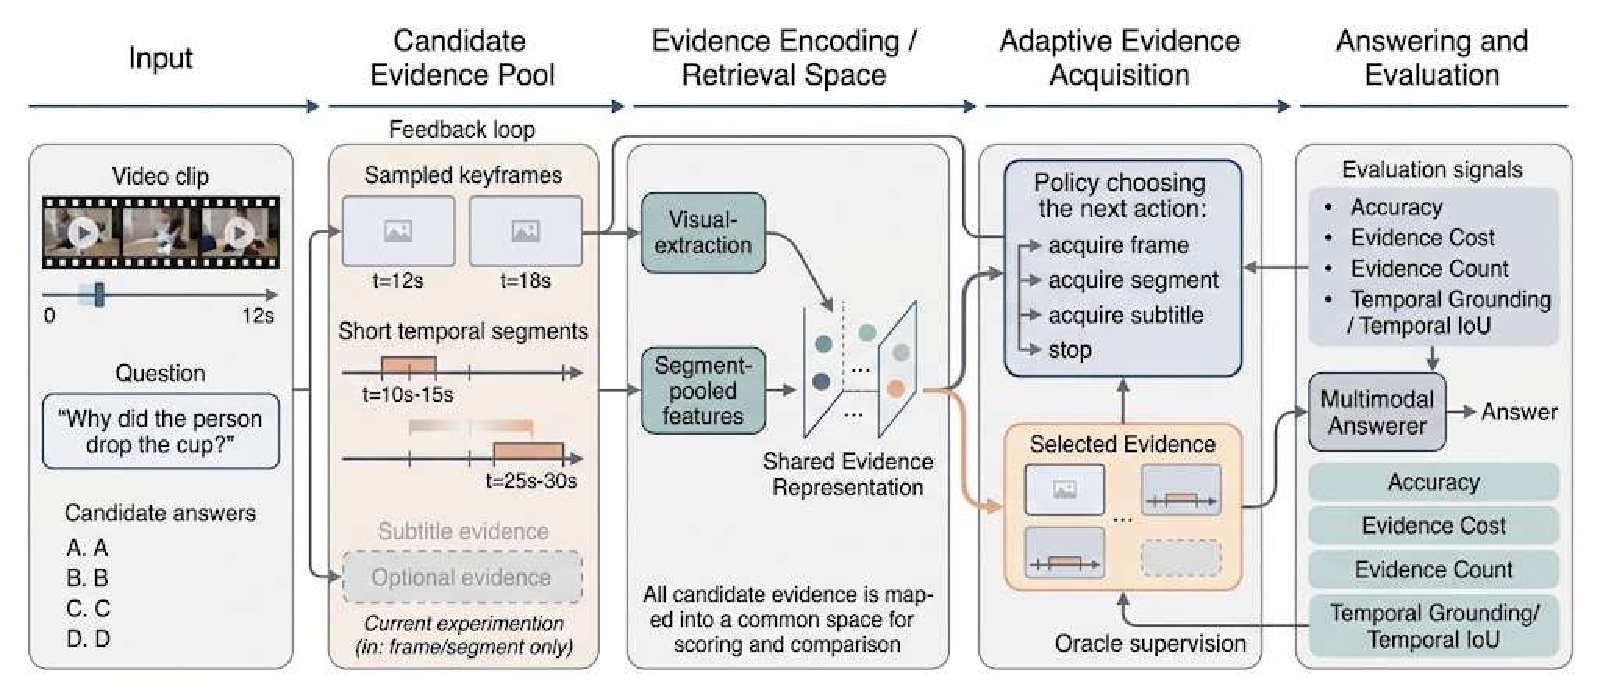
\includegraphics[width=\textwidth]{figure_1.pdf}
  \caption{Overview of the adaptive evidence acquisition pipeline. Candidate evidence is encoded into a shared space, a policy selects a compact subset under a budget, and the answerer is evaluated on answer quality, cost, and temporal grounding.}
  \label{fig:overview}
\end{figure}

Taken together, these trends suggest that multimodal retrieval alone is no longer an especially strong contribution. The more interesting question is how much evidence is actually needed, at what granularity, and under what budget. Our formulation is closest in spirit to retrieval-augmented video reasoning, but it shifts the objective from improving candidate recall to controlling how much evidence is ultimately consumed at inference time. Figure~\ref{fig:overview} summarizes this shift in emphasis: the point is not that retrieval is unimportant, but that retrieval alone does not resolve how much evidence a model should consume for a particular question. The initial NExT-GQA results reported later offer a first empirical signal in this direction, because the learned acquisition policy operates at a very different evidence budget from the fixed-budget baseline while maintaining comparable answer accuracy.

\section{Method}
The method proceeds in five stages. Raw dataset annotations are first converted into a unified example schema that stores the question, answer options, answer label, temporal grounding, and the metadata needed for later visual processing. A multimodal candidate pool is then built for each example. In the present NExT-GQA experiments, the main evidence sources are sampled frame candidates and short temporal segment candidates, and each evidence item is represented in a common structure containing modality, timestamps, retrieval score, and acquisition cost. This shared representation allows evidence types to compete inside one budgeted acquisition process rather than being handled by separate modality-specific pipelines. Real frame evidence is extracted from source videos using standard video processing tools, after which visual representations are computed for individual frames and segment-level representations are obtained by pooling features over short temporal windows. This provides a practical retrieval space without requiring full end-to-end video-language training.

The answering stage currently uses a frozen multimodal scorer built on CLIP-based retrieval features. For fixed-budget evaluation, a retriever collects a fixed number of items from each modality, and oracle traces are constructed by greedily pruning evidence while enforcing correctness and a minimum sufficiency constraint. Although this pruning procedure does not guarantee a globally minimal subset, it provides question-specific supervision that is aligned with the evidence preferences of the current answerer and is therefore practical for policy learning. These traces supervise the sequential acquisition policy and define which decisions should preserve answer quality under a budget. At each decision step, the policy conditions on the question, the evidence acquired so far, and the remaining budget, so acquisition becomes a sequential decision problem rather than a one-shot quota. The learned policy predicts whether to acquire subtitle evidence, frame evidence, segment evidence, or to stop. During policy learning and rollout, stopping is disallowed before at least one evidence item has been acquired; this prevents a trivial zero-evidence solution and ensures that the stop action represents a real budgeted decision rather than a bypass of the acquisition process. In addition, frames and segments carry different acquisition costs, so the policy is encouraged to trade local visual snapshots against broader temporal context rather than simply minimizing the number of selected items. In the current NExT-GQA experiments, subtitles are unused, so the effective competition is between frames and segments rather than the full subtitle-frame-segment setting planned for the larger study. This formulation matters because the goal is not merely to reduce compute, but to make evidence usage question-dependent: some questions appear to need multiple temporally distributed cues, whereas others can be resolved from a single highly informative visual observation. A fixed-budget strategy cannot express that distinction, while a sequential strategy can stop early when additional evidence is redundant and can expose the tradeoff between compactness and temporal grounding.

\section{Experiments and Preliminary Results}
Experiments are conducted on NExT-GQA, which is well suited to this study because it supports grounded VideoQA and exercises the full retrieval-and-acquisition pipeline on real videos. The present setting uses a 500-example training subset and a 200-example validation subset, with evidence restricted to frames and temporal segments. Retrieval is performed with a hybrid CLIP-based scoring scheme, answers are produced by a frozen multimodal scorer, and the learned policy chooses among acquiring frame evidence, acquiring segment evidence, and stopping. Learned-policy results are aggregated over three seeds (13, 21, 34). Because all methods share the same candidate pool, the same evidence encoder, and the same answer-scoring component, the comparison isolates acquisition behavior rather than conflating evidence selection with backbone changes. The same per-item acquisition costs and the same maximum budget are used throughout, so any difference in total evidence usage reflects a change in stopping behavior rather than a relaxed evaluation setting. The subset protocol is therefore intended as a controlled regime for validating the acquisition loop itself before scaling to larger runs.

The comparison includes three systems. The fixed-budget baseline retrieves three frames and three segments before answering with the frozen multimodal scorer. The keyword sequential policy serves as a heuristic control and, in the current setting, effectively consumes the same full allocation as the fixed-budget baseline. The learned sequential policy is a trainable linear controller over acquisition states, supervised by oracle traces derived from the same frozen multimodal answerer. All three methods therefore share the same candidate pools and answer-scoring component, so the main difference lies in the acquisition strategy itself rather than in the backbone or retrieval space. We report answer accuracy, selected evidence cost, selected evidence count, and selected temporal IoU. Together, these metrics capture the tradeoff between answer quality and evidence efficiency while retaining a grounding signal, and they help distinguish genuine evidence efficiency from cases where low cost is achieved only by sacrificing temporal relevance.

\begin{table}[t]
  \centering
  \scriptsize
  \caption{NExT-GQA results on a controlled subset of the train/validation splits. Learned-policy numbers are aggregated over three seeds.}
  \label{tab:nextgqa-results}
  \begin{tabular}{lcccc}
    \toprule
    Method & Accuracy & Cost & Count & Temp. IoU \\
    \midrule
    Fixed-budget baseline & 0.360 $\pm$ 0.000 & 7.5 $\pm$ 0.0 & 6.0 $\pm$ 0.0 & 0.273 $\pm$ 0.000 \\
    Keyword policy & 0.360 $\pm$ 0.000 & 7.5 $\pm$ 0.0 & 6.0 $\pm$ 0.0 & 0.273 $\pm$ 0.000 \\
    Learned policy & 0.365 $\pm$ 0.000 & 1.5 $\pm$ 0.0 & 1.0 $\pm$ 0.0 & 0.168 $\pm$ 0.000 \\
    \bottomrule
  \end{tabular}
\end{table}

The fixed-budget and keyword-policy baselines coincide in the current setup, so the meaningful contrast in Table~\ref{tab:nextgqa-results} is between fixed allocation and learned acquisition. The learned policy reaches 0.365 validation accuracy compared with 0.360 for the fixed-budget baseline while reducing the average evidence cost from 7.5 to 1.5 and the average evidence count from 6.0 to 1.0; given the 200-example validation split, the safest interpretation is that it \emph{matches} fixed-budget performance while using only about 20\% of the evidence cost. The zero variance across seeds reflects an effectively deterministic small-scale setting in which the candidate pools and oracle traces are fixed and the learned controller converges to the same operating point across random initializations.

\begin{table}[t]
  \centering
  \scriptsize
  \caption{Relative comparison against the fixed-budget baseline.}
  \label{tab:relative-results}
  \begin{tabular}{lcccc}
    \toprule
    Method & Acc. Ratio & Cost Ratio & Count Ratio & Temp. IoU Ratio \\
    \midrule
    Keyword policy & 1.000 & 1.000 & 1.000 & 1.000 \\
    Learned policy & 1.014 & 0.200 & 0.167 & 0.615 \\
    \bottomrule
  \end{tabular}
\end{table}

Table~\ref{tab:relative-results} makes the tradeoff explicit: relative to fixed budget, learned acquisition retains 1.014$\times$ answer accuracy while using 0.20$\times$ evidence cost and 0.167$\times$ evidence count, but only 0.615$\times$ temporal IoU. Read together, Table~\ref{tab:nextgqa-results} provides the absolute operating point and Table~\ref{tab:relative-results} highlights how far that operating point moves from a fixed-allocation regime. The overall picture is a different operating point rather than a minor gain: one selected item instead of six on average, similar answer accuracy, and weaker grounding overlap. This pattern is consistent with substantial redundancy in the fixed-budget candidate pool and supports the view that evidence selection should be treated as part of the model rather than as a fixed preprocessing choice. At the same time, the temporal-IoU drop is informative rather than incidental. It suggests that evidence efficiency is easier to obtain than faithful localization, which is precisely why answer accuracy, evidence cost, and grounding need to be reported together instead of as separate diagnostics.

The learned operating point is also interpretable in terms of evidence granularity. Under the current cost design, frames carry unit cost while temporal segments carry cost 1.5, so an average selected-evidence cost of 1.5 together with an average count of 1.0 indicates that the learned controller often prefers a single temporally extended item over a larger mixed bundle of frames and segments. This is a useful intermediate finding because it suggests that, for many questions in the current subset, short temporal context may be more valuable than accumulating multiple isolated visual snapshots. Whether this behavior persists with stronger answerers, subtitle evidence, and larger datasets is still an open question, but the present results already show that the policy is not simply reducing item count arbitrarily; it is moving the system toward a different temporal granularity of evidence.

\paragraph{Discussion and Future Work.} The present evidence is still limited in scope by the use of a frozen multimodal scorer, modality-level acquisition actions, and reduced grounding overlap, so the current results should be read as an encouraging operating-point study rather than as a complete validation of minimal sufficient evidence. The next stage will broaden the empirical analysis in three directions. First, we will scale the same protocol from controlled subsets to larger NExT-GQA runs and eventually the full train/validation splits in order to test whether the current accuracy-cost tradeoff survives outside the small-scale regime. Second, we will report oracle-validity, sufficiency, and comprehensiveness statistics directly, so that the minimal-evidence claim is supported by explicit evidence-preservation measurements rather than inferred only from compactness. Third, we will extend the study to stronger answerers and subtitle-aware grounded benchmarks, allowing us to test whether the current policy behavior reflects genuine redundancy in the evidence pool or only the operating characteristics of the present answerer. These experiments will also enable per-question-type analysis and qualitative visualizations of selected evidence, which should clarify when adaptive stopping is reliable and when larger temporal context remains necessary.

\clearpage
\bibliographystyle{plainnat}
\bibliography{references}

\end{document}
